\documentclass[8pt,a4paper]{article}
\usepackage[utf8]{inputenc}
\usepackage[T1]{fontenc}
\usepackage{amsmath}
\usepackage{amsfonts}
\usepackage[scale = 0.8]{geometry}
\usepackage{amssymb}
\usepackage{graphicx}
\usepackage{pdfpages}
\usepackage{hyperref}
\usepackage{float}
\usepackage{subfig}
\usepackage{tikz}
\usepackage{hyperref}
\usepackage{natbib}
\bibliographystyle{unsrtnat}
\usepackage{float}  

\usepackage{caption} %many figures in one figure (note subfigure and subfig are deprecated) 
%\usepackage{subcaption} %many figures in one figure (note subfigure and subfig are deprecated) 

\usepackage{latexsym}
\usepackage{parskip}
\usepackage{enumerate}

\title{\textbf{\LARGE GEOS 518} \\[1ex] Final project \\[1ex]  Simulating Tropical Cyclones over the South-West Indian Ocean with MPAS: Sensitivity to Boundary Layer schemes}
%\title{}
\author{Yao Gahounzo}

\begin{document}
	
	
	
	\maketitle
	
	
	
	%\textsc{\LARGE BOISE STATE UNIVERSITY}\\[1.5cm] 
	
	\section{Introduction} 
	
	Tropical cyclones (TCs) are a menace in many islands and coastal regions in the tropics, where TCs account for more than 40\% of economic losses and human deaths from natural hazards. The strong winds, heavy precipitation, storm surges, and massive floods make TCs a deadly force of nature \citep{oguejiofor2019simulating}. The devastating impacts of the TCs are usually severe in the coastal communities along the South West Indian Ocean (SWIO), where Madagascar, Mozambique, Zimbabwe, and South Africa are mostly affected. Some tropical cyclones that made landfall over these countries have destroyed farmlands (pushing farmers to debts), fell power lines (causing electrocutions; \citep{oguejiofor2019simulating}), collapsed buildings, rendered thousands of people homeless \citep{fitchett201466}, displaced communities (\url{https://www.worldvision.org/disaster -relief-news-stories/}), and even killed people \citep{fitchett201466}. The TC Kenneth, which occurred between the 21st to  28th of April 2019, is one of the most deadly TCs. The TC Kenneth, which can be rated as the second most intense TC (i.e., after TC Idai), affected four countries (Mozambique, Malawi, Comoros, and Zimbabwe). Kenneth displaced about 3.8 million people (including 185,000 people in Comoros and 199,836 people in Mozambique), caused more than one billion US dollars damages, and killed about 52 people (\url{https://reliefweb.int/disaster/tc-2019-000038-moz}).
	
	
	The damages caused by extreme winds and coastal flooding when cyclones made landfall \citep{singh2017impact} can be significantly reduced with reliable forecasts of the cyclone system. We used the Model for Prediction Across Scales (MPAS), which allows very high-resolution simulations in local and global terms to simulate TC. The MPAS model allows us to draw up the problems encountered at the poles' level in the simulation of atmospheric phenomena.  An accurate tropical cyclone model must consider cloud convection, wind speed, sea surface temperature, boundary layer (PBL), the lowest (1-3 km) of the atmosphere, among other processes. The BL is an interface between the troposphere and the ground, and its flow is dominated by turbulent eddies. The BL is well known for its essential role in developing and maintaining TCs since it exchanges momentum, moisture, wind, heat, and water vapor with the earth's surface through the transfer of turbulence from the air mass.
	
	Given the importance of the BL in describing the atmospheric phenomena, especially in TC description, PBL schemes have been developed into climate and weather forecasting models. The two predominant PBL schemes in the MPAS model, the Yonsei University scheme (YSU) and Mellor-Yamada-Nakanishi-Niino (MYNN) scheme, have been used to investigate the causes and evolution of these extreme events.
	
	This study aims to evaluate the capability of the MPAS in the simulation of the TC Kenneth and examine the sensitivity of the simulation to the PBL schemes.
	
	The specific objectives of the study are as follows:
	
	\begin{itemize}
		
		\item Study the characteristic of the TC Kenneth.
		\item Evaluate how well MPAS simulate the characteristic of TC Kenneth.
		\item Study the sensitivity of the simulated TC Kenneth to BL schemes in MPAS.
	\end{itemize}
	
	
	
	\section{Data }
	
	The data used for model initialization were downloaded from the NCEP Climate Forecast System Version 2 (CFSv2) 6-hourly Products \citep{cisl_rda_ds094.0}. The dataset contains analyzed atmospheric, oceanic, and land surface products and forecasts. The main data used are the SST data downloaded from 21st to 28th April, 2019, the surface and pressure data combined in a single file for the first 6 hours of April 21, the day TC Kenneth started.  These data formats are the WMO GRIB2, and the variables are recorded in the variables table (Vtable) described on the dataset site.
	
	The observational data used for the comparison with the model was obtained from the Regional Specialized Meteorological Centre (RSMC) of Météo-France \citep{meteofr2019data}. RSMC supplied data every 6 hours, including the maximum wind speed, minimum sea level pressure (MSLP), and the location (latitude and longitude) of the MSLP of TC Kenneth. The reanalysis data was obtained from the ERA5 data set (\url{https://cds.climate.copernicus.eu/cdsapp#!/search?type=dataset}).
	
	
	\section{MPAS description}
	
	\subsection{Overview}
	
	
	The model used in this study is the MPAS model, a global model that has the ability to increase the resolution to simulate TC over a region of interest. It is a set of components to simulate the Earth system and consists of MPAS-Atmospheric core, MPAS-Ocean core, MPAS-Land ice core and MPAS-Sea ice core (\url{https://mpas-dev.github.io/}). It is distinguished by the use of unstructured Voronoi meshes and discretization of the C grid to overcome the limitations of global models on regular grids and allowed variable resolutions across the globe with smooth transitions between different zones of refinement. 
	The atmospheric component of MPAS (MPAS-A) is a global non-hydrostatic model. The two prominent components incorporated in MPAS-A are atmospheric dynamics and physics; and an initialization component to generate the conditions of the state of the atmosphere and the Earth's surface (\url{https://mpas-dev.github.io/}). 
	
	
	\begin{figure}[H]
		\centering 
		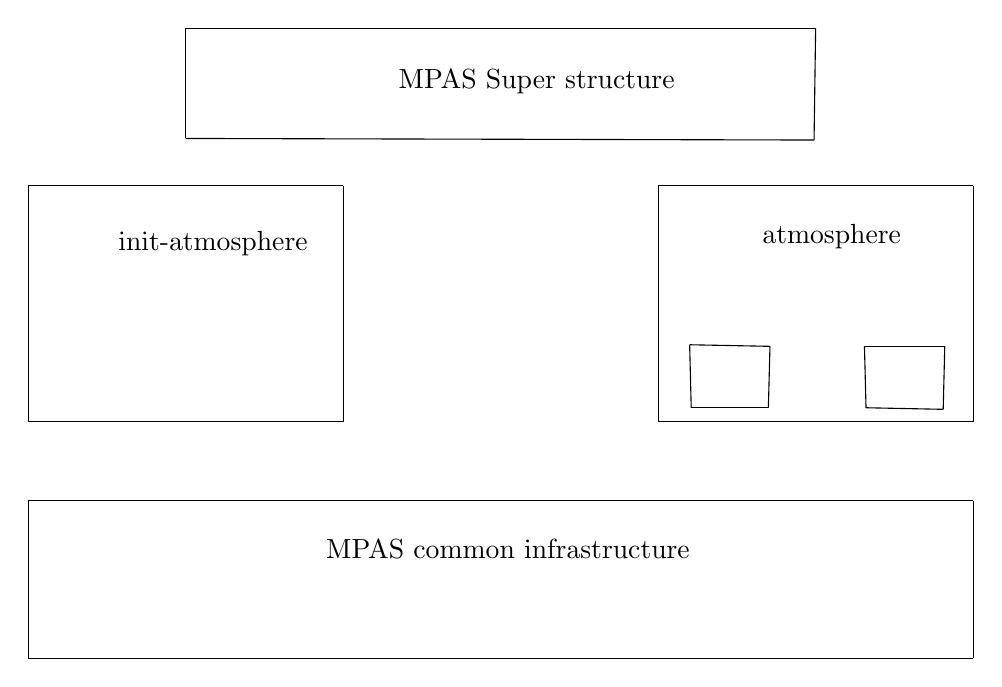
\begin{tikzpicture}%[line cap=round,line join=round,>=triangle 45,x=1.0cm,y=1.0cm]
			%\clip(-4.3,-3.06) rectangle (23.38,11.02);
			\draw  (0.,8.)-- (8.,8.);
			\draw  (8.,8.)-- (7.98,6.58);
			\draw  (7.98,6.58)-- (0.,6.6);
			\draw  (0.,6.6)-- (0.,8.);
			\draw  (-2.,6.)-- (2.,6.);
			\draw  (2.,6.)-- (2.,3.);
			\draw  (2.,3.)-- (-2.,3.);
			\draw  (-2.,3.)-- (-2.,6.);
			\draw  (6.,6.)-- (6.,3.);
			\draw  (6.,3.)-- (10.,3.);
			\draw  (10.,3.)-- (10.,6.);
			\draw  (10.,6.)-- (6.,6.);
			\draw  (-2.,2.)-- (10.,2.);
			\draw  (10.,2.)-- (10.,0.);
			\draw  (10.,0.)-- (-2.,0.);
			\draw  (-2.,0.)-- (-2.,2.);
			\draw  (6.4,3.98)-- (7.42,3.96);
			\draw  (7.42,3.96)-- (7.4,3.18);
			\draw  (7.4,3.18)-- (6.42,3.18);
			\draw  (6.42,3.18)-- (6.4,3.98);
			\draw  (9.64,3.96)-- (9.62,3.16);
			\draw  (9.62,3.16)-- (8.64,3.18);
			\draw  (8.64,3.18)-- (8.62,3.96);
			\draw  (8.62,3.96)-- (9.64,3.96);
			\draw (2.58,7.6) node[anchor=north west] {MPAS Super structure};
			\draw (-0.98,5.54) node[anchor=north west] {init-atmosphere};
			\draw (7.2,5.64) node[anchor=north west] {atmosphere};
			\draw (1.66,1.64) node[anchor=north west] {MPAS common infrastructure};
			\draw  (0.,8.) ;
			\draw  (8.,8.);
			\draw  (7.98,6.58) ;
			\draw  (0.,6.6);
			\draw  (-2.,6.) ;
			\draw  (2.,6.) ;
			\draw  (2.,3.) ;
			\draw  (-2.,3.) ;
			\draw  (6.,6.) ;
			\draw  (6.,3.) ;
			\draw  (10.,3.) ;
			\draw  (10.,6.) ;
			\draw  (-2.,2.) ;
			\draw  (10.,2.) ;
			\draw  (10.,0.) ;
			\draw  (-2.,0.) ;
			\draw  (6.4,3.98) ;
			\draw  (7.42,3.96) ;
			\draw  (7.4,3.18) ;
			\draw  (6.42,3.18) ;
			\draw  (9.64,3.96) ;
			\draw  (9.62,3.16) ;
			\draw  (8.64,3.18) ;
			\draw  (8.62,3.96) ;
			
		\end{tikzpicture}
		\caption{The initial and model component of MPAS}
	\end{figure} 
	
	
	\subsection{MPAS-Atmosphere meshes and grid-rotate}
	
	MPAS-A consists of centroidal spherical Voronoi meshes that allow high-resolution global simulations using either quasi-uniform resolution or a configuration of horizontal meshes with variable resolution. The Spherical centroidal
	A voronoi tessellation (SCVT) mesh decomposition file with an appropriate number of partitions is required to run the MPAS-A; therefore, a limited number of mesh decomposition files are provided within each mesh. The models have different mesh resolutions, e.g., 60-15 km, 60-3 km, 92-25 km, and others. The number of grid cells varies widely depending on the configuration, e.g., 535554 for 60-15 km mesh resolution, 835586 for 60-3 km mesh, and 163842 for a mesh resolution of 92-25 km. Each variable resolution mesh is provided with a region of refinement that is centered on $0^{\circ}$ latitude and  $0^{\circ}$ longitude. The grid-rotate program allows the rotation of an MPAS mesh file from one geographic location to another. The usefulness of grid rotation is the need to save computing resources due to the considerable amount of time it can take to prepare an SCVT mesh, especially a mesh with many generation points or a high degree of refinement. Figure \ref{fig:ff} shows the rotation of the MPAS mesh file to our area of study, SWIO.
	
	\begin{figure}[H]
		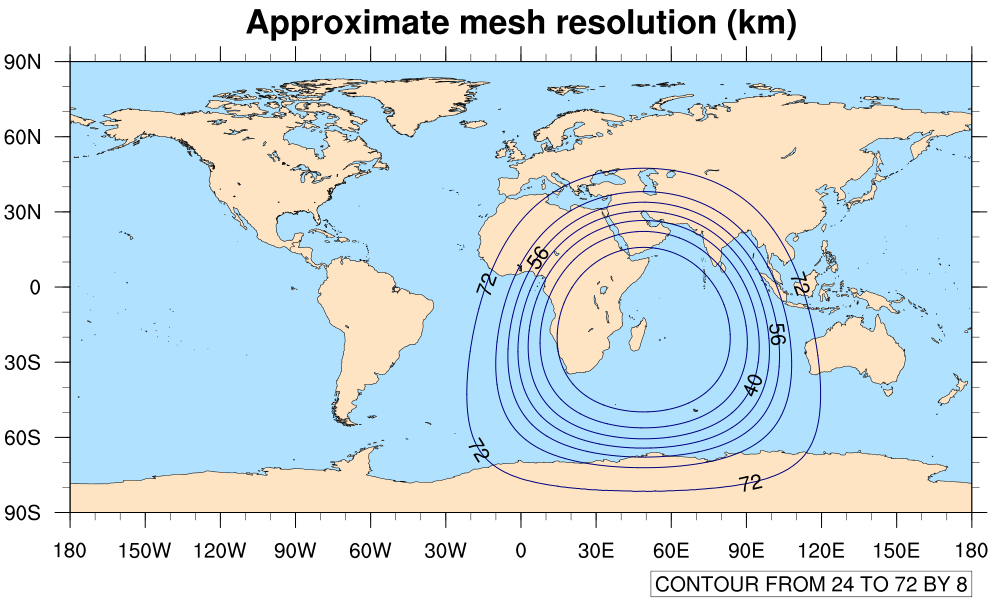
\includegraphics[width = \linewidth]{mesh_resolution1.png}
		\caption{Rotation of the mesh variable resolution over the area of study, SWIO.}
		\label{fig:ff}
	\end{figure}
	
	
	\section{MPAS configuration}
	
	
	
	Our simulation is performed using version 6.0 of MPAS-A.  A quasi-uniform resolution of a 240 km grid was used for the simulation test. The configuration of the global variable resolution of the grid, which is refined from 25 km to 92 km, is used in the evaluation of the MPAS.  The model is used for an 8-days simulation period from 21st to 28th April 2019, during which Kenneth TC occurs. The model simulation uses 41 vertical levels up to 30 km and a sample output rate of 6-hourly data. Due to the high resolution of the simulations and the limitations of computing resources, two simulations were performed with MPAS-A. The first experiment uses the YSU scheme as in WRF 3.8.1, in the default mesoscale physics reference suite in MPAS-A, and the second experiment was performed using the MYNN scheme as in WRF 3.6.1. As YSU is part of the default physics suite, it is used in most studies and was the largest  PBL scheme evaluated in the MPAS. The choice of MYNN is to evaluate and analyze its results against the default results and show which scheme best describes the BL in the TC simulation. The physics of the model operates on cell-centric variables, and for the horizontal moment, they use the $u$ component of the wind and the $v$ component of the wind. The physical trends of the horizontal winds are produced at the center of the cells and are projected to the edges to update the horizontal moment. For graphics and visualizations, the NCAR command language (NCL) built from Fortran 90 was used.
	
	\begin{table}[H]
		\centering 
		%\renewcommand{\arraystretch}{1.3}
		%\newcolumntype{C}{>{\centering\arraybackslash}m{5cm}}
		\begin{tabular}{p{7cm}|p{7cm}}
			\hline 
			\multicolumn{2}{c}{\textbf{Detail}}\\\hline
			Grid Resolution &92-25 km\\
			Vertical levels&41\\
			&\\
			\textbf{Physics schemes}& \\
			Convection scheme& New Tiedtke\\
			Micro-physics scheme& Wsm6\\
			Planetary Boundary Layer Scheme& YSU/ MYNN\\
			Short wave radiation Scheme& RRTMG\\
			Long wave radiation Scheme &RRTMG\\
			Cloud fraction for radiation& Xu-Randall\\
			Surface Layer scheme&Monin-Obukhov\\\hline
		\end{tabular}
		\caption{Model configuration detail.}
	\end{table}
	
	To examine atmospheric and oceanic conditions during the lifetime of TC Kenneth, observational data (OBS) and the MPAS model output were used to determine the 10-m maximum wind speed, vorticity, and the minimum sea level pressure (MLSP) along the Kenneth's track. The intensity of the TC is characterized by the MSLP and maximum wind speed; therefore, they are taken into account throughout this work to assess the intensity of the cyclonic system.
	
	For the evaluation of the sensitivity of the two schemes YSU and MYNN in the TC Kenneth simulation, the MPAS was run with both schemes separately from 21 April at 00h00 to 28 April at 18h00, and were compared to the observation and reanalysis in terms of track, 10-m maximum wind speed, and MSLP. The 10-m maximum wind speed and MSLP variables were presented as time series to allow analysis on a time scale.
	
	
	
	\section{Track and evolution of tropical cyclone Kenneth}
	Figure \ref{fig:4.1} validates the 8 days of stimulation with MYNN and YSU, and shows the tracks for the reanalysis, observation and the simulated models of the TC Kenneth. 
	The storm center of the stimulated track is detected by locating the MSLP using the TC detection algorithm.
	While the reanalysis and MYNN show southward divergence on the first day of the simulation, the reanalysis can accurately reproduce the track of the TC for the remainder of its lifetime.
	The simulation with YSU shows a consistent track with the observational data from the first day and the first 12 hours of the second day of the simulation. Between $41^{\circ}$E and $52^{\circ}$E, the northward bias in the track presented by YSU to the observation can be explained by the strong wind ($11.70 m/s$) of the TC with YSU at the beginning compared to the observation ($10.27 m/s$). However, the path presented by YSU landfall closer to where the observation landfall in Mozambique. Compare to the observation and reanalysis, the MYNN has a northward bias between $41^{\circ}$E and $49^{\circ}$E. There are discrepancies on the TC Kenneth category between the observation that presents the cyclone up to category 4 to the other data which presents only tropical storm in Saffir-Simpson Scale. This may be due to the northward shift in the simulation affected by the Coriolis force weakening towards the equator. The storm for the experiments intensifies from tropical depression to tropical storm during the bias period. This variation in the location of the low pressure may be the possibility of the bias observation. The track given by MYNN shows that the cyclone makes landfall further south ($14^{\circ}$S) than the others ($13^{\circ}$S). Compare MYNN landfall time to the reanalysis and observation it makes landfall 6h. The figure shows that the models simulated, reanalysis, and the observation start at the same day but at different location, and the position of YSU in 25th is behind that of the observation. This may be due to lack of accuracy in the tracking algorithm. 
	The models simulated do not capture well the TC track and this may be attributed to poor model resolution or lack of detail in the boundary conditions \citep{mohanty2010simulation}.
	
	
	\begin{figure}[H]
		\centering 
		\includegraphics[width = 12cm]{N/K_track_HDN}
		\caption{Figure showing the track followed by the Tropical cyclone Kenneth from the 21st of March to the 28th of April 2019: (red) represented the observation, (green) the reanalysis, (yellow) MYNN, and (blue) YSU. The numbers 21, 25, and 28 represent the date at which the TC reaches the location }.
		\label{fig:4.1}
	\end{figure}
	
	Figure \ref{fig:4.2} shows the evolution of the MSLP and maximum wind speed. In panel (a), the simulation experiments generally have higher MSLPs compared to observation and reanalysis from 21 to 23 April. 
	Both schemes follow the same low-pressure pattern until 24 April, but MYNN reaches its peak at the same period as observed with $993.13 hPa$ and $934 hPa$, and with tropical storm and category 4 respectively on the 25th. Since MYNN made landfall before the observation, its pressure gradually increases to about $1007.93 hPa$ as its intensity decreases. Reanalysis and YSU reach their maximum before and after the observation and MYNN, but the reanalysis MSLP is lower than the MYNN, and MSLP of YSU is observed on the 25th April 6h before the observation reaches its peak with $989.61 hPa$.
	The temporal evolution of the observational data depicts that after TC Kenneth reached the peak on the 25th and made landfall at the same time, it deteriorated rapidly due to the entanglement of dry air it encountered over land, which explains the increase in MSLP values from $975 hPa$ to $1002 hPa$. In general, MYNN has low MSLP values compared to YSU. However, the schemes could not represent well the intensification of TC Kenneth. They are not able to reproduce MSLP values as lower as the observation.
	
	\begin{figure}[H] 
			\centering
			\subfloat[\centering ]{{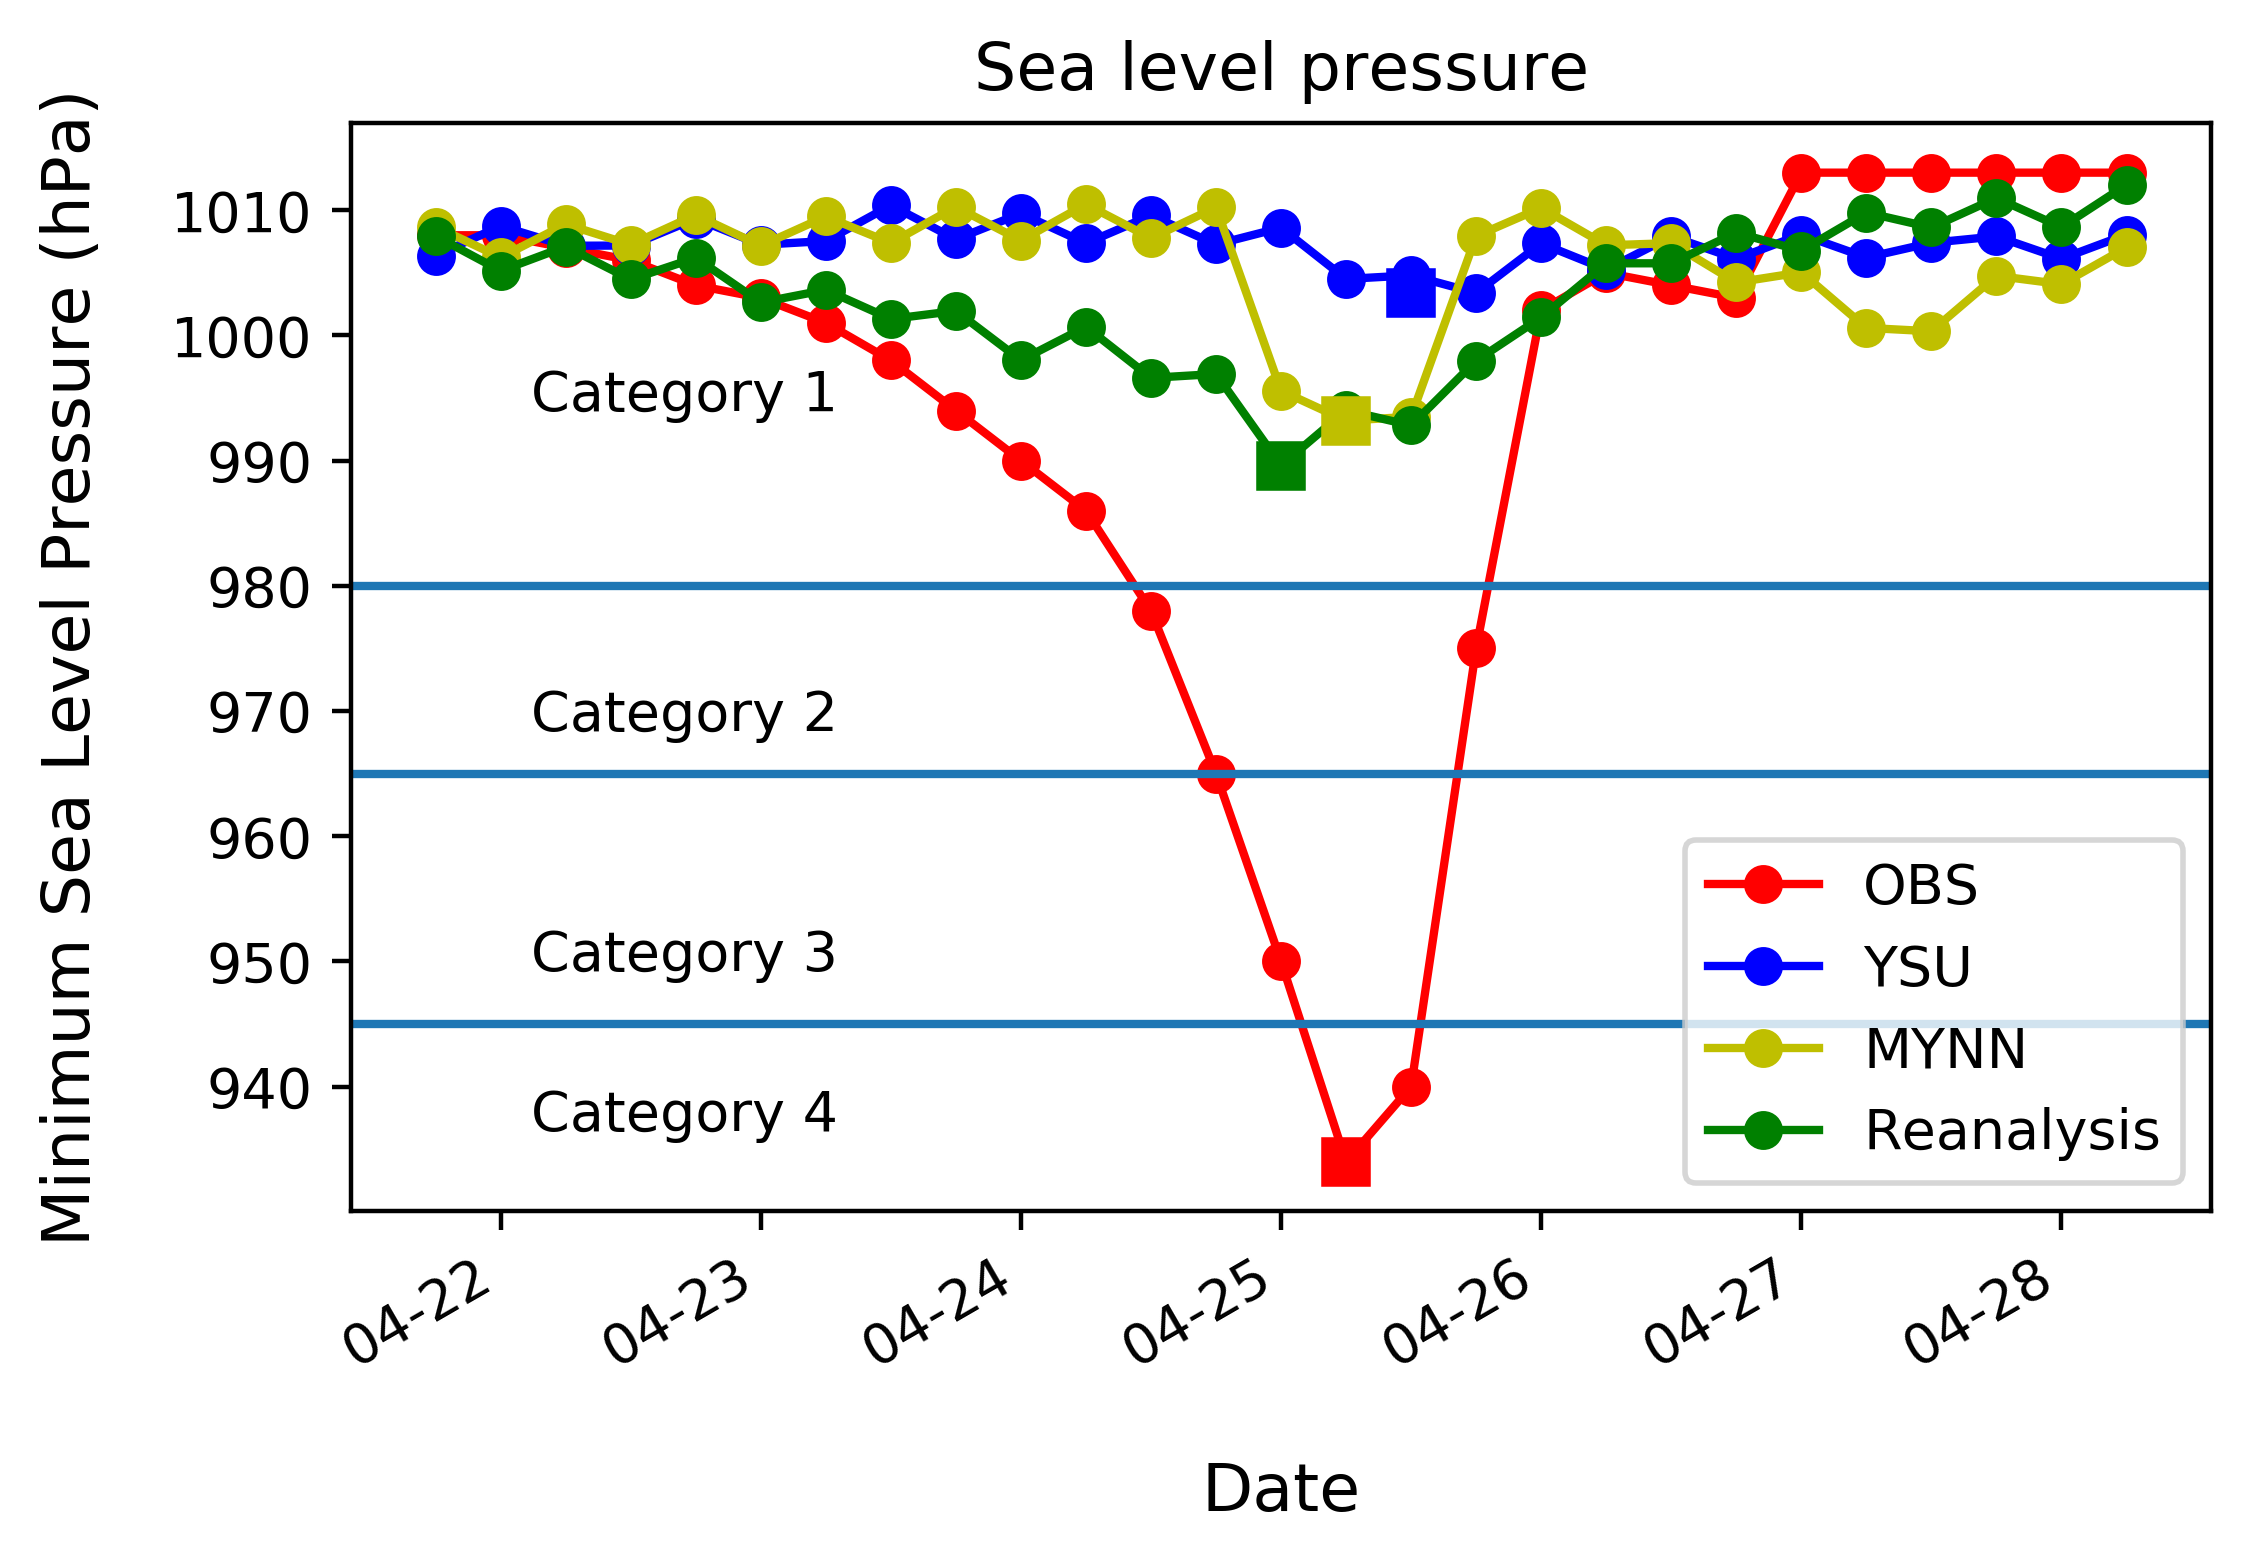
\includegraphics[width=8cm]{images/MSLP_y} }} 
			\subfloat[\centering ]{{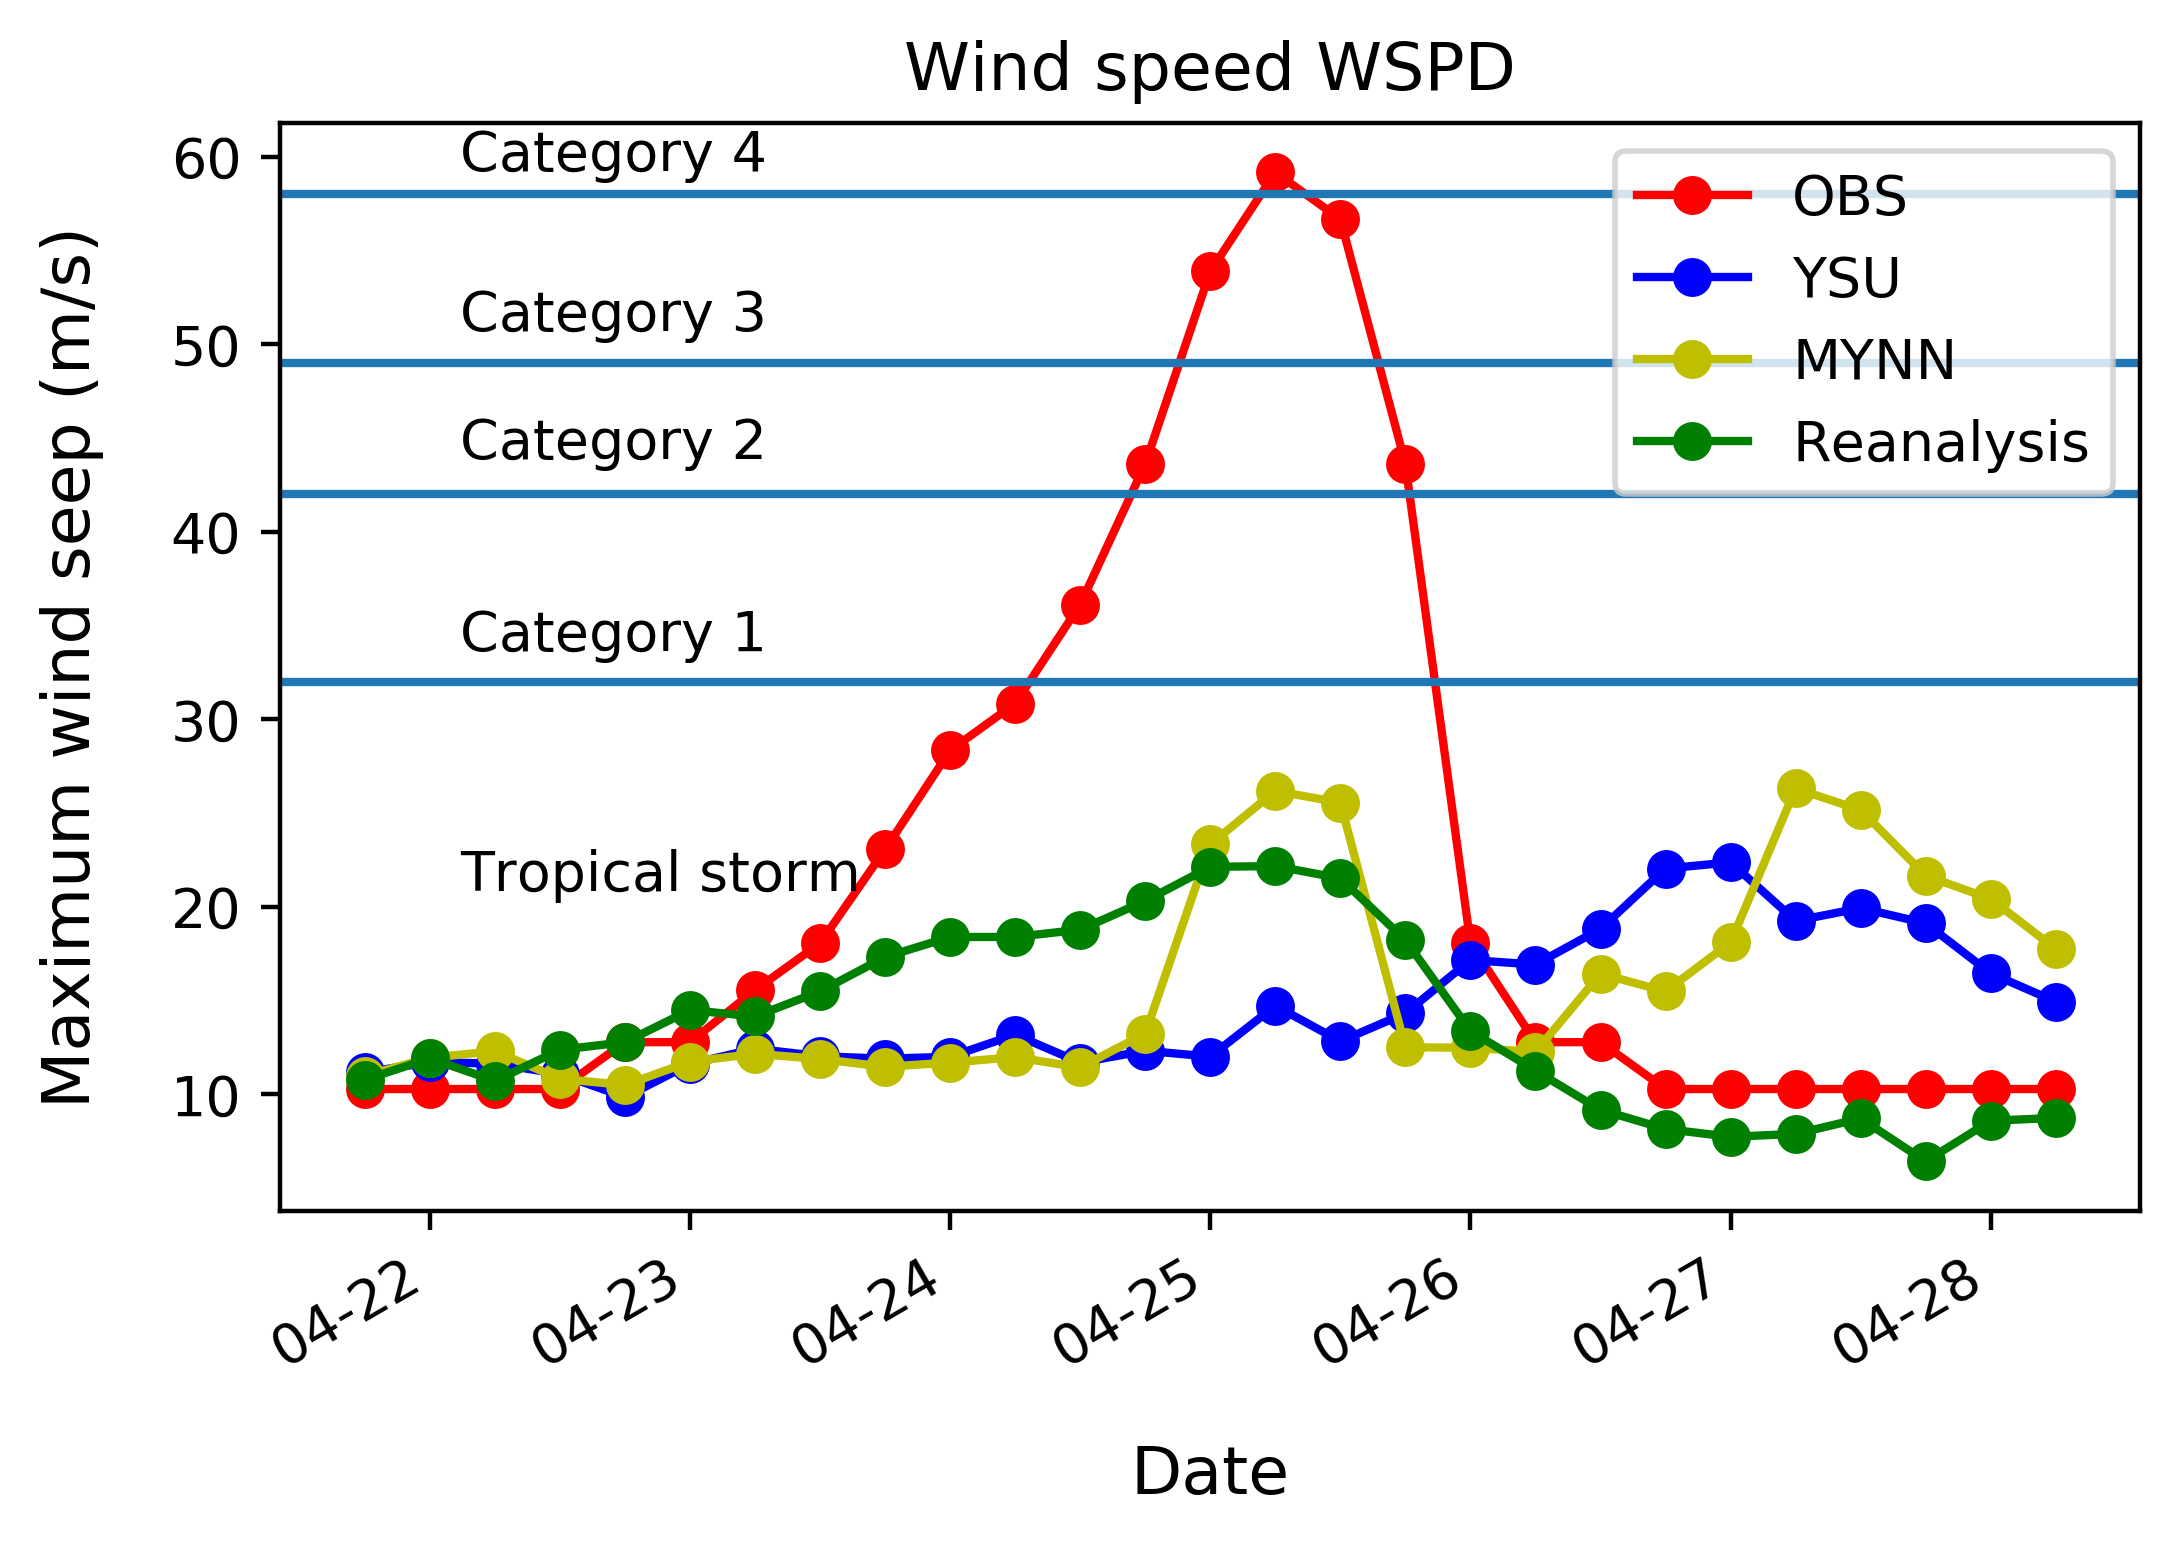
\includegraphics[width=8cm]{images/WSPD_y}  }}
		\caption{Figure showing the evolution of the Tropical Cyclone Kenneth from the 21st of March to the 28th of April 2019: (a) Mean Sea Level Pressure, and (b) Wind Speed.}
		\label{fig:4.2}
	\end{figure}
	
	
	Wind speed is one of the features that characterize the intensity of the TC. Figure \ref{fig:4.2}.b shows the temporal evolution of the wind speed of TC Kenneth and shows that the cyclone acquire its highest wind speed ($59.16 m/s$) on April 25th at 06h00, which places it in category 4. By examining the graphs, one realize that the model simulations do not follow the same magnitude of the wind speed compare to the observation but the speed is rapidly increased for the MYNN which allows it to reach its peak on the 25th at 06h00 as the observation with $26.17 m/s$. From the reanalysis and YSU it can be seen that TC Kenneth acquire its maximum wind speed at a different period from the observation and in the case of the reanalysis it quickly became weak after reaching that peak.
	The reanalysis gives a reasonable performance of TC Kenneth wind speed compare to the MYNN that follows approximately the observed data from the first two days of the system development but in terms of intensity MYNN perform better. The failure of the simulations to properly capture the observation may be due to the late and early landfall of YSU and MYNN on 25th  and 26th respectively , and also to the model resolution.
	
	We realize that for both variables that characterize the intensity of TC, the models simulated failed to capture the intensity of the TC Kenneth. This may be attributed to inadequate physical parameterizations, the inaccuracy of tracking and detection algorithm or the poor model resolution.
	
	

	\section{Structure of the simulated Tropical Cyclone}
	
	Figures \ref{fig:4.4}  represent the dynamical structure of the TC Kenneth. This includes warm core in the storm center, eye in the center of the cyclone and strong winds near the eyewall.
	
	To investigate the sensitivity of the TC structure to BL, figure \ref{fig:4.4} shows the simulated horizontal wind speed on the day the cyclone reaches its peak for MYNN on April 25th at 06h00, YSU on April 25th at 18h00, and the reanalysis on April 25 at 00h00. It shows that the experiments are in remarkable agreement with the reanalysis, but a considerable variation in wind speed was observed. The MYNN has a maximum wind speed of about $26 m/s$ on its peak day, and it is higher than the reanalysis and the YSU wind speed of about $21 m/s$. Figure \ref{fig:4.4} were represented the wind and warm core of the cyclone. The figure clearly identifies the cyclonic flow moving from the north to the south, and the strongest winds were observed in the East than the West. The wind is moving clockwise around the low pressure, and since the direction of TC is a phase, it has the same direction as the background flow and is the addition of the cyclonic and background flow. The observation of the strongest wind in East than West is explained by the background flow acting in the same direction as the cyclonic flow in East but blowing against the background in the West. In panel (b) of the figure \ref{fig:4.4}, the speed observed around the center is stronger compared to that of reanalysis and YSU, but the warm core is less relative to others in panels (a) and (c).
	

	\begin{figure}[H]
		
		
		\centering
		\subfloat[\centering ]{{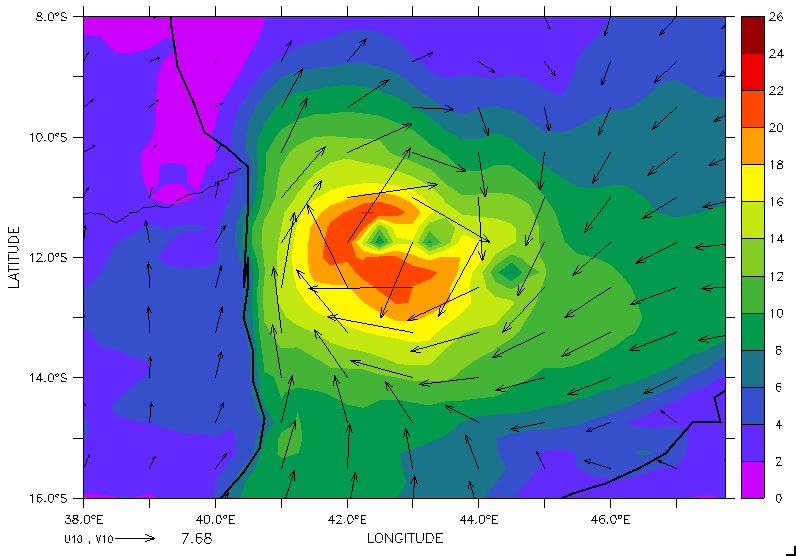
\includegraphics[width=8cm]{new_image/w_RR} }}%
		
		\subfloat[\centering ]{{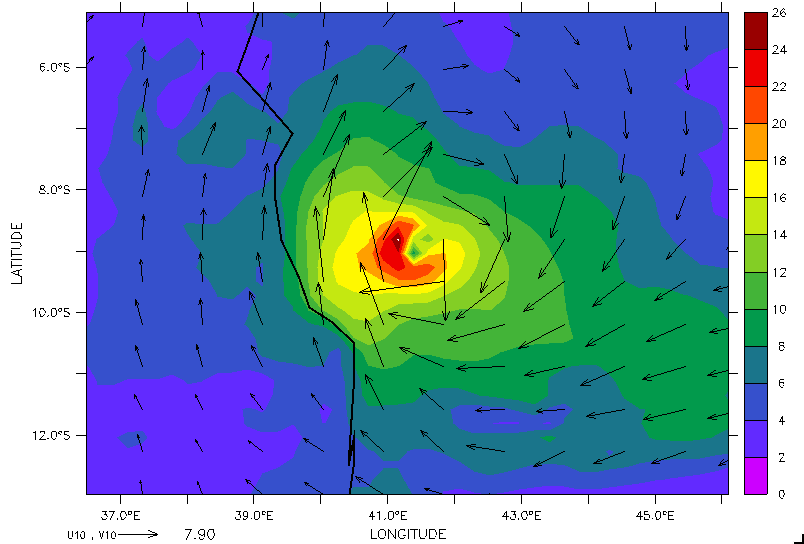
\includegraphics[width=8cm]{new_image/w_M26} }}%
		\subfloat[\centering ]{{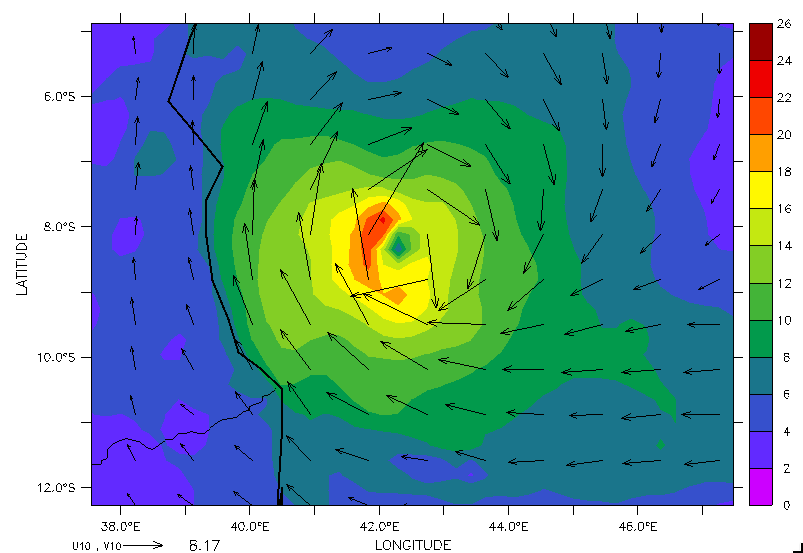
\includegraphics[width=8cm]{new_image/w_Y} }}%
		\caption{Dynamical structure of Tropical Cyclone Kenneth at the peak day: panel (a) shows the wind speed for the reanalysis, (b) shows the wind speed for MYNN, and (c) shows the wind speed for YSU}
		\label{fig:4.4}
	\end{figure}


	\section{Conclusion}
	
	The present work focused on the reliability of the MPAS model to simulate TC Kenneth by using a variable grid resolution of 92-25 km. The emphasis was made on the MYNN, and YSU schemes to study the BL impact on the cyclonic system. To achieve this, the analysis focused on some of the TC characteristics such as track, wind speed, MSLP, and vorticity.
	
	The results show how PBL schemes impact the dynamic variables especially, MSLP and wind speed during the TC intensification phase. From the discussions, it became clear that before the intensification phase the schemes do not have a significant impact on the intensity and tracks but allow a clear structure of the cyclone. The structure is adequately produced during its peak day.
	
	During the intensification of the cyclone simulated with YSU which defaults to the mesoscale suite and MYNN, different variations are observed in the tracks and dynamic variables such as MSLP and wind speed.
	
	Overall, MYNN presented a cyclone structure that follows the observation and reanalysis but with a notable divergence that may be due to oceanic conditions especially in the Mozambique channel where TC Kenneth developed.
	
	The reanalysis produced well the tracks while the MPAS model simulated with the schemes produce a strong bias in the tracks and the dynamic structure of the cyclone. The schemes gave a remarkable characteristic of the eye and the eye wall during their peak days but they underestimated the value of the different variables. 
	
	
	\newpage 
	\bibliography{references}
	
\end{document}